\documentclass[a4paper,12pt]{elsarticle}
\usepackage{graphicx}
\usepackage{hologo}
\usepackage{amsmath}
\usepackage{caption}
\usepackage{verbatim} % for comments
\usepackage[table,xcdraw]{xcolor}
\usepackage[utf8]{inputenc}
\usepackage{hyperref}
\usepackage{float}
\usepackage[section]{placeins}
\begin{document}

\begin{frontmatter}

\title{Importance of Multidisciplinary Design Optimization for Wave-Driven Desalination Systems}

\author{Nate DeGoede$^a$, Maha Haji$^a$}

\affiliation[a]{Department of Mechanical Engineering, University of Michigan, Ann Arbor, MI, USA}

\begin{abstract}
This is the abstract. Summarize your problem, approach, and key results concisely. You can include equations and references if needed.
\end{abstract}

\end{frontmatter}

\section{Introduction}
The global freshwater crisis necessitates innovative solutions for clean water production. Demand for freshwater is anticipated to grow by over 40\% by 2050 \cite{watershortage2015}, while droughts, urbanization, and uneven distribution of water resources add to the pressure on our existing freshwater supplies. Seawater reverse osmosis (SWRO) is a proven technology for creating freshwater from seawater, but is quite energy intensive, requiring 2-4 kWh/m$^3$ \cite{Li2018}. This cost associated with this high energy demand make up 25\%-40\% of the total cost of water \cite{blue_econ}, and when supplied through fossil fuels, this energy consumption further exacerbates water scarcity challenges \cite{nytdrought}. To ensure sustainability, it is therefore crucial to power SWRO efficiently through renewable energy sources.

Various renewable energy sources for powering SWRO, such as wind \cite{GarciaRodriguez2001} and solar \cite{Elkadeem2024}, have been explored. Another intriguing solution is wave energy converters (WECs). SWRO and WECs have natural co-location, with SWRO plants typically situated near the coast while WECs are deployed offshore. Beyond both being marine-based technologies, WECs and SWRO plants share complementary operational characteristics \cite{blue_econ}. SWRO requires high pressure seawater, and WECs can provide this directly using a hydraulic style power take-off (PTO) system, forming a wave driven desalination system \cite{Davies2005}. This direct drive approach eliminates the need for conversion to an intermediate form of energy, potentially improving overall system efficiency and reducing system complexity. This has the potential to give WECs a significant advantage over other renewable energy sources for powering SWRO desalination.

Despite their potential, WECs face significant challenges limiting their widespread adoption. Notably, their high costs pose a major barrier. Therefore, design optimization is essential to improve economic viability. Multidisciplinary Design Optimization (MDO) provides a systematic framework to address this challenge by simultaneously considering the designs and interactions of multiple subsystems and optimizing overall performance rather than isolated improvements \cite{Sobieski}. MDO approaches integrating PTO design with hydrodynamics and/or controls has been demonstrated to significantly improve the design of electricity producing WECs \cite{Stroefer2023,PenaSanchez2022,Rosati2023,Grasberger2024}. Michelén Ströfer et al. (2023) see a 22\% increase in electrical power output through PTO and control co-design (CCD) \cite{Stroefer2023}, while Grasberger et al. (2024) report a 60\% improvement in performance using MDO when compared to traditional design methods \cite{Grasberger2024}. 

The application of MDO to these problems is effective because of the interactions between the WEC, PTO, and SWRO plant. In 2016 Garcia-Rosa and Ringwood \cite{GarciaRosa2016} investigated the sensitivity of optimal WEC geometry to control strategy, demonstrating the importance of control co-design. Coe et al. have further advanced our understanding of these interactions through impedance matching studies. In 2021 Coe et al. demonstrated how well-established control techniques, causal feedback control and impedance matching, are quite effective for WEC control, but requires a well designed PTO system that properly shapes the system impedance \cite{Coe2021}. In 2025, Coe et al. tackle this challenge and apply impedance matching to PTO design \cite{Coe2025}. Although the studies by Coe et al. focus on rack and pinion style WEC PTOs for electricity generation, which do not have any rectifying behavior (unlike hydraulic PTOs like what are used in wave-driven desalination systems), impedance matching principles are important to consider for systems with rectifying behavior too \cite{Ladan2015}.

These MDO and impedance matching studies emphasize the importance of utilizing holistic models that account for wave dynamics, PTO performance, and control strategies in electricity-generating WEC optimization. Despite this, these ideas have yet to be applied to wave-driven desalination systems, leaving a critical gap in research.

Yu and Jenne (2017  and 2018) \cite{YJecon2017,Yu2018},  Brodersen et al. (2022) \cite{brodersen2022}, Suchithra et al. (2022) \cite{Suchithra2022} and Simmons and Van de Ven (2023) \cite{Simmons2023} have all built models that account for the coupled dynamics of wave-driven desalination systems. However, these studies simply evaluate these systems and do not leverage their models for design optimization. 

This paper addresses this gap through the development of a holistic MDO framework for wave-driven desalination system design. A simplified wave-driven desalination schematic is shown in Figure \ref{fig:WDDS}, where an oscillating surge wave energy converter (OSWEC) drives a hydraulic cylinder, pressurizing seawater and delivering it to an onshore SWRO desalination plant. This system enables freshwater production without the need for major external energy input. While similar systems have been studies in literature \cite{Yu2018,Suchithra2022,Mi2023,Simmons2023}, this study has a notable difference in that it lacks an energy recovery unit (ERU).

\begin{figure}[]
    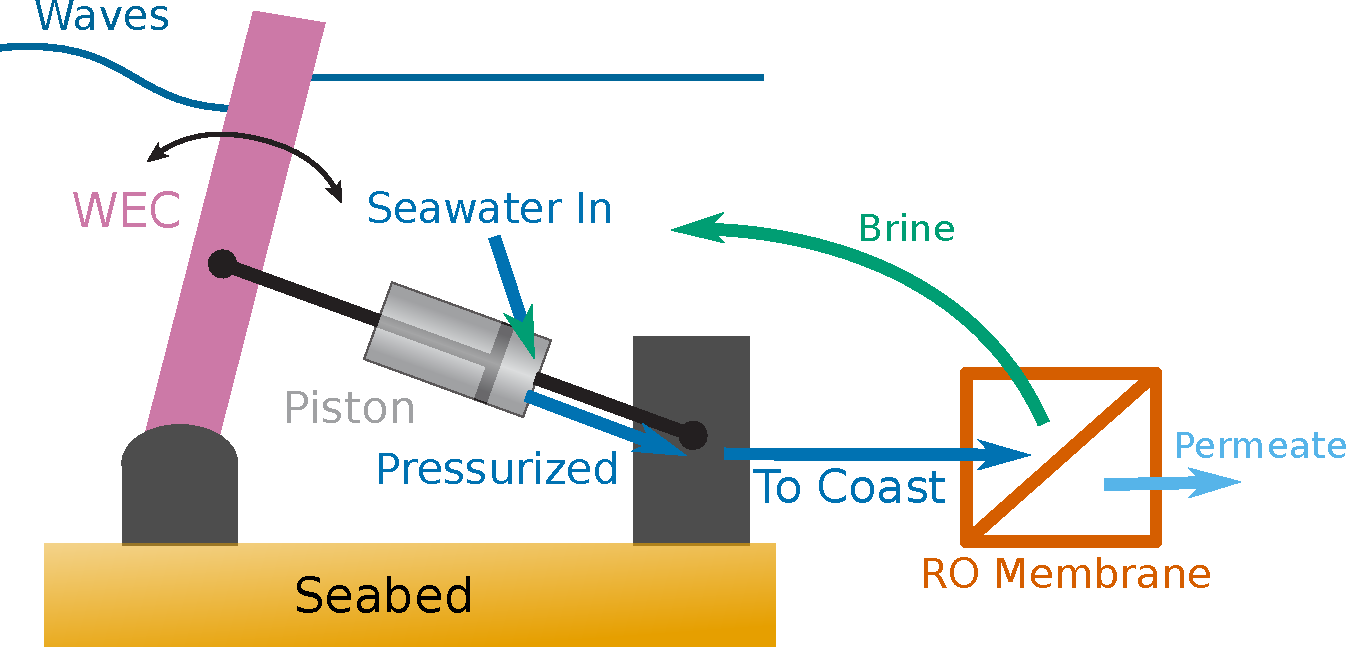
\includegraphics[width=\linewidth]{../figs/wdds.pdf}
    \captionof{figure}{Simple wave-driven desalination system concept sketch.}
    \label{fig:WDDS}
\end{figure}

The concept sketch (Figure \ref{fig:WDDS}) depicts a high level overview of the wave-driven desalination system but does not capture all the hydraulic components included in this design study. A detailed hydraulic circuit diagram is shown in Figure \ref{fig:hydraulics}, which includes an accumulator to smooth the pressure delivered to the SWRO plant, a pressure relief valve to avoid operating the SWRO plant beyond its rated capacity, a brine side throttle valve set to control the recovery ratio of the SWRO plant, as well as directional valves.

\begin{figure}[]
    \centering
    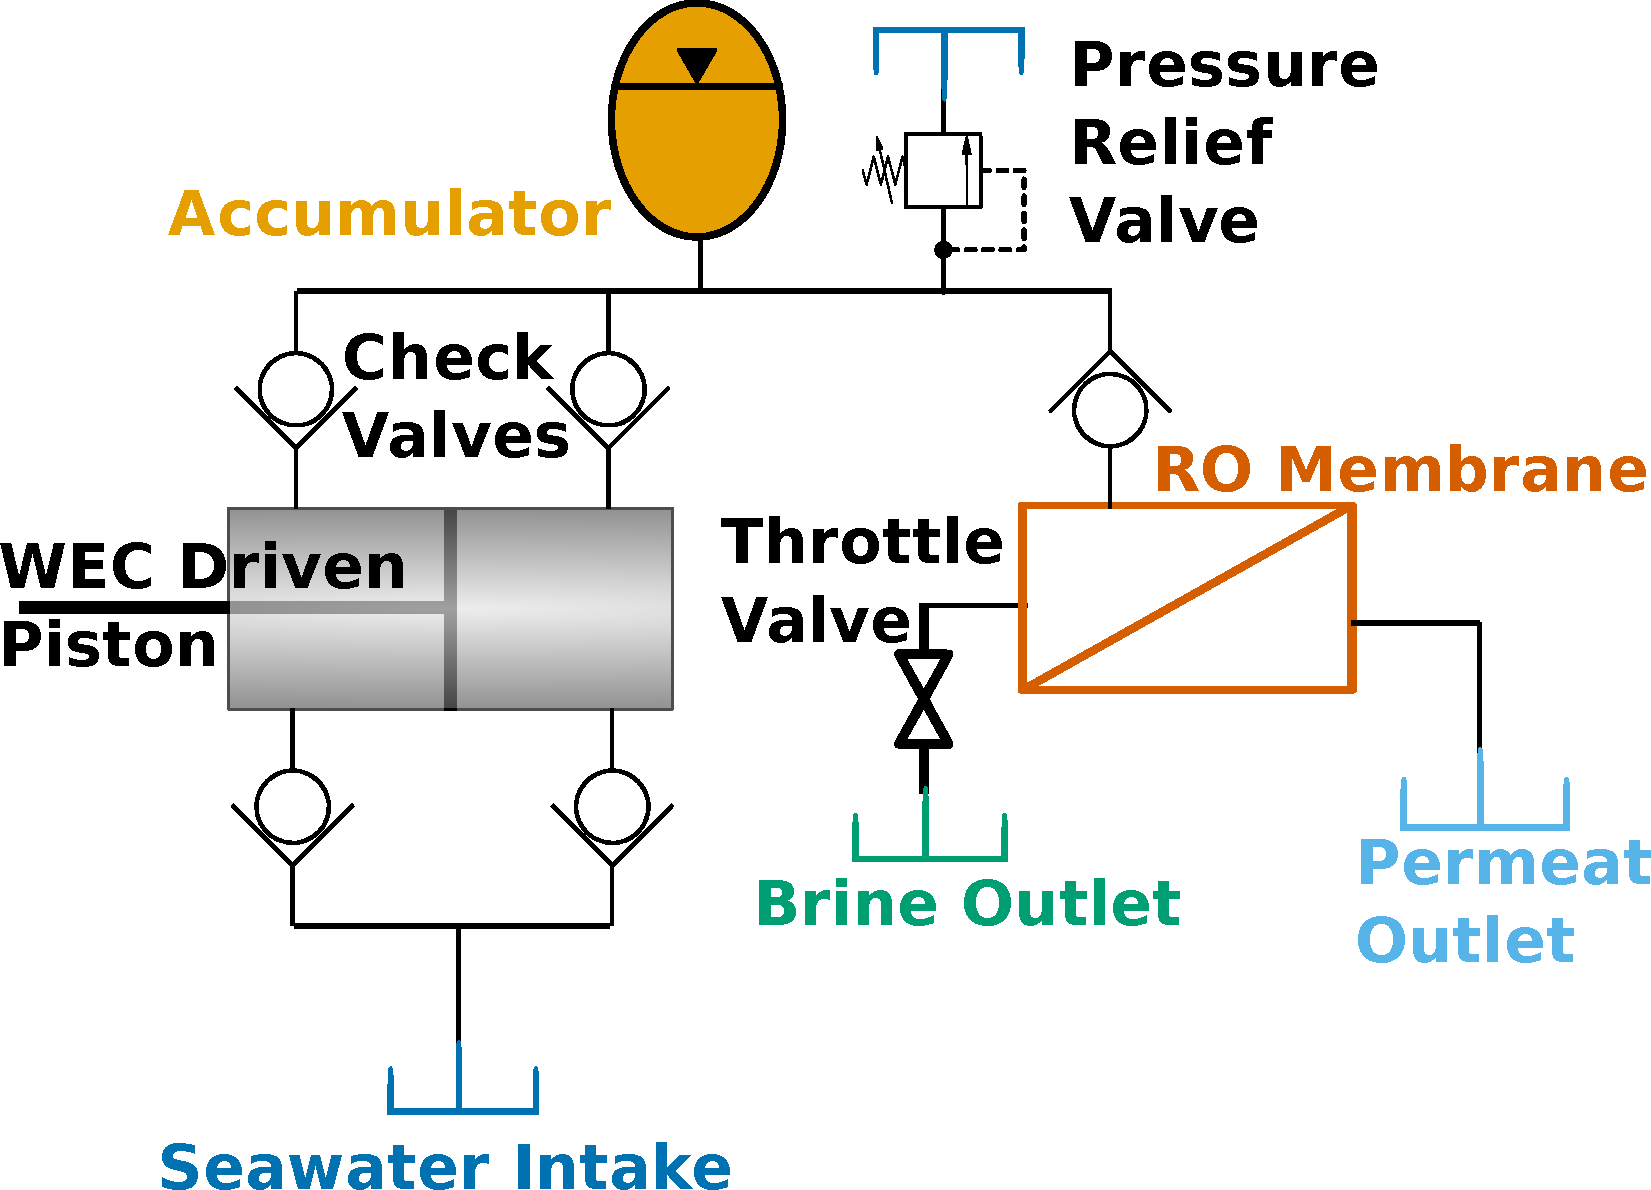
\includegraphics[width=0.7\linewidth]{../figs/hydraulic_circuit.pdf}
    \captionof{figure}{Hydraulic circuit diagram of the wave-driven desalination system.}
    \label{fig:hydraulics}
\end{figure}

One of the important design trade-offs to consider for these systems is the size of the accumulator vs the capacity of the SWRO plant. A larger accumulator offers more smoothing of the flow delivered to the SWRO plant. Since the SWRO plant can not operate above a certain capacity, a larger accumulator therefore allows for a smaller SWRO plant to be used without losing water through the pressure relief valve. Since the SWRO plant a major cost driver for the system \cite{YJecon2017}, investing in larger more expensive accumulators appears to be a massive cost saving strategy. However, as Michelén Ströfer et al. (2023) show, changing the impedance of the PTO system has a significant impact on the performance of a WEC \cite{Stroefer2023}. Therefore, it is important to consider the impact changing the accumulator size has on the system dynamics while making these economic trade-offs.

In addition to the higher usage rate argument, another common argument for large accumulators is that SWRO traditionally operates at steady state conditions. Lai et al. (2016) investigate the effectiveness of various smoothing methods for wind powered SWRO \cite{Lai2016}. Hopkins et al. (2014) do a similar study for wave-driven desalination, looking at various accumulator geometries \cite{Hopkins2014}.  However, the study by Hopkins et al. do not investigate the impact of accumulator design on WEC performance, ignoring the interactions between the WEC and PTO. Bacelli et al. (2009) \cite{Bacelli2009} developed a controller to minimize pressure fluctuations in a wave-driven desalination system, and do consider the coupled dynamics of the WEC and PTO, but do not consider the trade-offs between smoothing and overall system performance. However, a more recent study by Sitterley et al. (2022) \cite{Sitterley2022} shows that unsteady operation of SWRO is feasible and not as detrimental to membrane performance as typically feared. This finding opens the design space to investigate systems with less smoothing, although admittedly more research is needed to fully understand the techno-economic implications of unsteady SWRO operation.

When optimizing WEC systems, the optimal design of the device is highly dependent on the assumed wave conditions. Robertson et al. (2022) show that optimal WEC geometry is fundamentally dependant on the incident wave spectrum \cite{Robertson2022}. Due to the variability in incident wave conditions even at a single location, it is important to consider a variety of sea states when optimizing WEC systems. Many studies consider a variety of sea states when optimizing WEC systems, for example Stroefer et al. (2023) \cite{Stroefer2023} use a weighted average of the performance across multiple sea states as their objective function. This study takes a different approach by optimizing the design fort various sea states individually, giving us a better understanding of the sensitivity of the optimal design to sea state. 

This paper demonstrates the importance of wholistic modeling and co-design for wave-driven desalination systems. In Section \ref{sec:problem}, our formal MDO problem formulation is presented, defining our design space and an overview of the wholistic model. Section \ref{sec:model} goes into detail on the models for the various disciplines considered. Section \ref{sec:results} presents the results of our optimization studies which are then discussed in Section \ref{sec:discussion}. Finally, conclusions and future work are presented in Section \ref{sec:conclusion}.

\section{Problem Formulation} \label{sec:problem}
\subsection{Multidisciplinary Design Optimization Framework}
The optimization problem in this study is formally defined as:
\begin{align*} 
    \text{Minimize} \quad & \text{LCOW}(\mathbf{x},\mathbf{p}; \hat{u})  \\
    \text{by varying} \quad & \mathbf{x}\\
    \text{subject to} \quad &  \mathbf{g} \leq 0 \\
    \text{while solving} \quad & \mathbf{R}(\mathbf{x},\mathbf{p};\hat{u}) = 0\\
    \text{for} \quad & \hat{u}
    \label{eq:problem}
\end{align*}
\noindent LCOW (levelized cost of water) is the objective function (discussed further in Section \ref{sec:econ}). The design vector, $\mathbf{x}$, contains variables related to WEC, PTO, and SWRO plant, summarized in Table \ref{tab:design_space}. The vector, $\mathbf{p}$, contains parameters related to environmental conditions and fixed design choices (shown in \ref{app:params}). $\hat{u}$ represents the coupled variables solved for by $\mathbf{R}$, the governing equations of the various disciplinary modules: geometry, seawater desalination, hydrodynamics, system dynamics, and economics. The problem is subject to inequality constraints ($\mathbf{g}$) related to the piston motion and pressure which are enforced in the system dynamics module, Section \ref{sec:sysdyn}.

\begin{figure*}
    \centering
    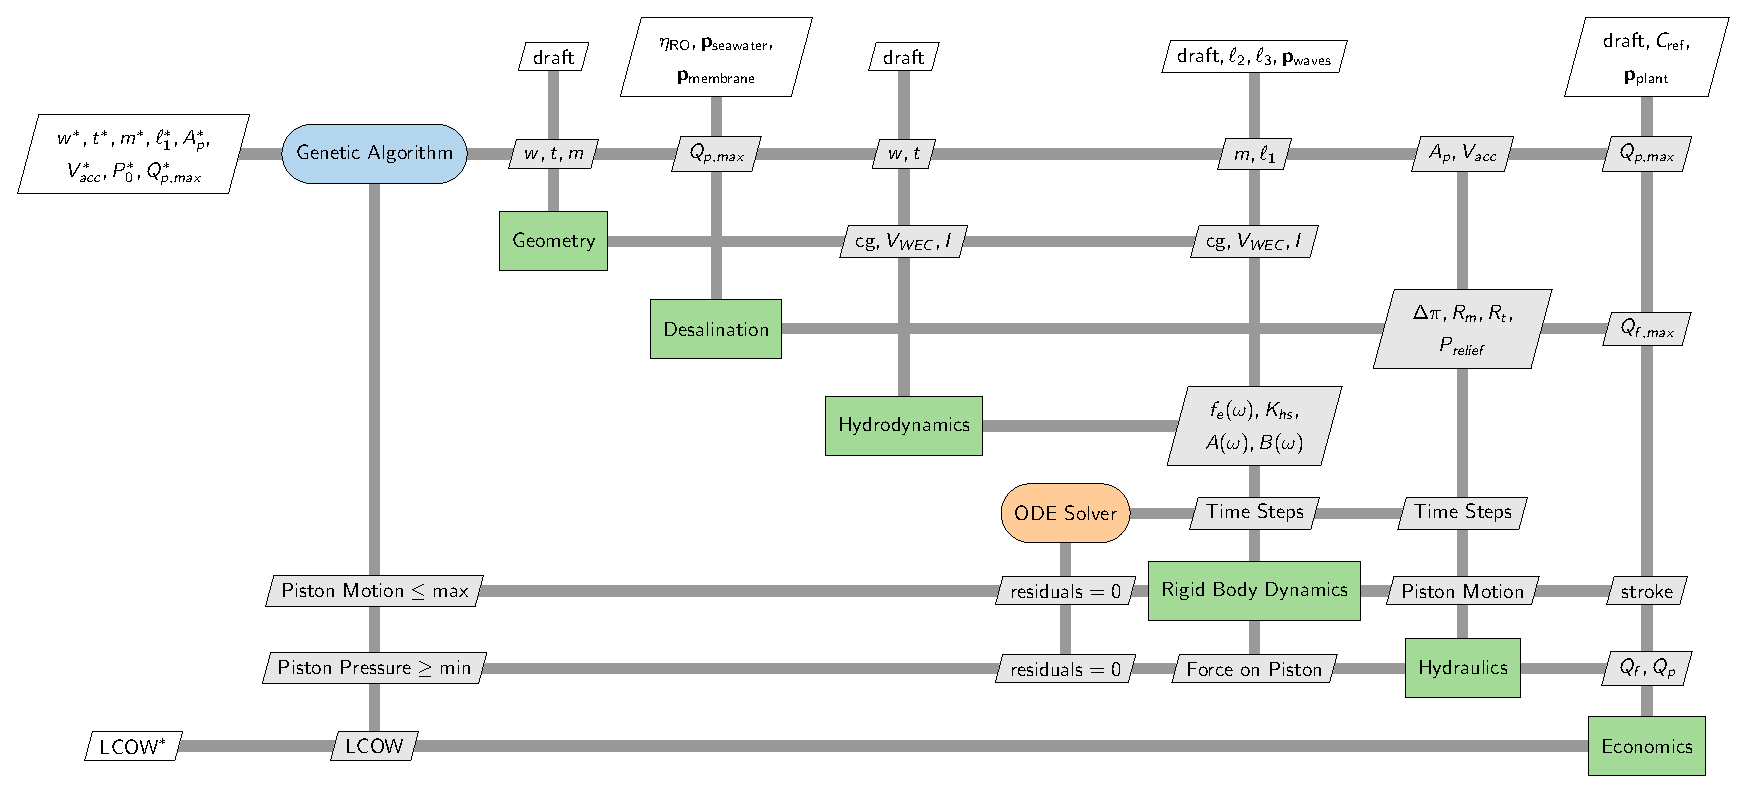
\includegraphics[width=\linewidth]{../figs/xDSM_merged.pdf}
    \captionof{figure}{xDSM diagram of the wave-driven desalination system optimization problem. Note $\mathbf{p}_\text{seawater}$, $\mathbf{p}_\text{membrane}$, $\mathbf{p}_\text{waves}$, and $\mathbf{p}_\text{plant}$ represent vectors of parameters related to the membrane, seawater, sea state, and desalination plant architecture respectively.}
    \label{fig:xdsm}
\end{figure*}

Figure \ref{fig:xdsm} presents a graphical representation of the MDO problem using an Extended Design Structure Matrix (xDSM) \cite{xdsm}. The diagram uses gray line to illustrate the flow of information between the disciplinary modules and optimizer, while gray parallelograms indicate module inputs and outputs. The white parallelograms show optimizer level inputs and outputs. 

\subsection{Design Space} 

\begin{table}[h]
    \centering
    \caption{Design Variables}
    \begin{tabular}{cccc}
        \hline
        Variable & Nominal Value & Lower Bound & Upper Bound\\
        \hline
        $w$ & 18 m & 10 m & 30 m \\
        $t$ & 2 m & 1 m & 5 m \\
        $m$ & 127$\times10^3$ kg & 50$\times10^3$ kg & 500$\times10^3$ kg \\
        $\ell_1$ & 2 m & 0.1 m & draft \\
        $A_p$ & 0.26 m$^2$ & 0.01 m$^2$ & 1 m$^2$ \\
        $V_{acc}$ & 4 m$^3$ & 0.01 m$^3$ & 6 m$^3$ \\
        $P_0$ & 3 MPa & 1 MPa & 7 MPa \\
        $Q_{p,max}$ & 3150 m$^3$/day & 1000 m$^3$/day & 10000 m$^3$/day\\
        \hline
    \end{tabular}
    \label{tab:design_space} 
\end{table}

A summary of the design space is shown in Table \ref{tab:design_space}. WEC variables consist of the width, $w$ [m], thickness, $t$ [m], and mass, $m$ [kg], of the OSWEC. PTO variables include the OSWEC hinge to PTO joint length, $\ell_1$ [m], piston area, $A_p$ [m$^2$], accumulator volume, $V_{acc}$ [m$^3$], and accumulator pre-charge pressure, $P_0$ [MPa]. Finally, the SWRO plant variable is the maximum plant production rate, $Q_{p,max}$ [m$^3$/day]. Many of these variables can be visualized in Figure \ref{fig:dvs}.

\begin{figure}
    \centering
    
\includegraphics[width=\linewidth]{../figs/dvs.pdf}
    \captionof{figure}{WEC (a) and mechanism (b) dimensions. Note that $h$ represents the WEC height, which is a parameter rather than a design variable.}
    \label{fig:dvs}
\end{figure}

It is important to note that some design parameters are not included in the design space. WEC height and draft is set to fixed value, as are mechanism variables $\ell_2$ and $\ell_3$. These were fixed to reduce design space dimensionality, as the other variables included provide sufficient control of the system dynamic characteristics (notably hydrodynamic stiffness, inertia, and excitation force, as well as the mechanical advantage of the mechanism). 

\subsection{Parameters and Constraints}
This study largely uses parameters similar to those used by Yu and Jenne (2018) \cite{Yu2018}. Full tables of parameters can be found in \ref{app:params}. Constraints are applied to device stroke length, maximum pressure in the hydraulic circuit, and minimum pressure in the piston cylinder. These are all enforced in the system dynamics module, Section \ref{sec:sysdyn}.

\subsection{Optimization Algorithm}
Due to the absence of accessible gradients in the hydrodynamics and system dynamics modules, a genetic algorithm (GA) is utilized. A table of GA hyperparameters is provided in \ref{app:params}.

\subsection{Sequential Design Optimization Approach}
MDO can be a computationally intensive task, which can limit its potential applications. In an effort to gage the importance of MDO for this specific application a comparison is made between MDO and sequential design optimization (SDO) approaches. In SDO, we will optimize the design of each subsystem (WEC, PTO, and SWRO plant) sequentially. To optimize the WEC design, we optimize for levelized cost of WEC kinetic energy [\$/kWh] when excited at the peak period and disconnected from PTO. The only costs associated with this are the WEC costs.

To optimize the PTO and SWRO plant designs, we take two approaches. The first approach optimizes the PTO for levelized cost of flow [\$/m$^3$] with the SWRO plant (membrane and pressure relief valve) replaced with a simple throttle valve. This results in optimizing the PTO to deliver the maximum feedflow into the SWRO plant at the lowest PTO cost. This PTO is then used in the optimization of the SWRO plant, which optimizes the SWRO plant design for LCOW.

The second approach chooses a nominal PTO design from literature \cite{Yu2018} and optimizes the SWRO plant design for LCOW using this fixed PTO design. This optimal SWRO plant design is then fixed while optimizing the PTO design for LCOW.

\subsection{Sensitivity Analysis}
The optimal design of the wave-driven desalination system is expected to change with different sea states. Since one of the goals of this study is to explore ares of potential design improvement through MDO, it is therefore important to see if the same design trends are present in a variety of sea states. To this end, optimizations are performed for 20 different sea states. The 20 sea states are selected using K-means clustering \cite{Arthur2007}. First, K-means clustering is performed on data from National Oceanographic and Atmospheric Administration (NOAA) National Data Buoy Center (NDBC) \cite{ndbc} for 5 different buoys. The 5 buoys locations chosen are: Guam (52200), Hilo HI (51206), Santa Monica Bay (46221), San Juan PR (41053), and Georges Bank (44011). 10 clusters are created for each buoy using hourly data from 2015-2024. From these 50 clusters, K-means clustering is performed again to create 20 final clusters used in the sensitivity study.

\section{System Modeling} \label{sec:model}
The xDSM in Figure \ref{fig:xdsm} shows the 5 primary disciplinary modules: ``Geometry'', which maps WEC design variables to geometric properties, ``Desalination'', which calculates the system dynamic properties of the SWRO plant, ``Hydrodynamics'', which determines various hydrodynamic coefficients, ``System Dynamics'', which solves the coupled dynamics of the wave-driven desalination system, and ``Economics'', which calculates the LCOW of the system. The ``Geometry'' module is straightforward and will not be discussed further. The remaining four modules are discussed in detail in the following subsections. This model framework was also presented and published by DeGoede and Haji (2025) \cite{idetc2025}.

\subsection{Desalination Module} \label{sec:desal}
The desalination module determines key SWRO plant parameters for a single-stage plant. It considers the capacity of the plant in addition to membrane parameters and seawater composition. The governing equation for the reverse osmosis process is:
\begin{equation}
    \label{eq:ro}
    Q_p = A_w A_m (\Delta P - \Delta \pi),
\end{equation}
\noindent where $Q_p$ is the permeate flow rate [m$^3$/s], $A_w$ is the water permeability coefficient [m$^3$/N-s], $A_m$ is the total membrane area [m$^2$], $\Delta P$ is the pressure difference across the membrane [Pa], and $\Delta \pi$ is the osmotic pressure difference across the membrane [Pa]. This osmotic pressure difference is calculated using \cite{separationprocesses}:
\begin{equation}
    \label{eq:osmotic_pressure}
    \pi = iCRT,
\end{equation}
\noindent where $i$ [-] is the number of ions produced per molecule of solute, $C$ [mol/m$^3$] is the concentration of the solute, $R$ [J/K-mol] is the ideal gas constant, and $T$ [K] is the temperature. For simplicity, $\Delta \pi$ is set as the osmotic pressure of the seawater minus the osmotic pressure of the target permeate concentration. A better model would consider the time variant concentrations on both sides of the membrane, but is outside the scope of this study.

The water permeability coefficient ($A_w$) is set to a constant value, matching the work by Yu and Jenne (2018) \cite{Yu2018}. This constant value is dependent upon membrane selection, for this paper we chose to use the same membrane as Yu and Jenne (2018), the SW30HR-380 Dry from DuPont \cite{SW30HR380}. Membrane area $A_m$ is set by calculating the amount of SW30HR-380 area is required to meet the SWRO plant capacity design variable, $Q_{p,max}$:
\begin{equation}
    A_m = \frac{Q_{p,max}}{Q_0}A_0,
    \label{eq:membrane_area}
\end{equation} 
\noindent where $Q_0$ and $A_0$ are the single-unit production and membrane area for the SW30HR-380 membrane, found on the datasheet \cite{SW30HR380}.

Next, for convenience a membrane resistance ($R_m$ [MPa-s/m$^3$]) is defined as: 
\begin{equation}
    \frac{1}{A_w A_m}
    \label{eq:membrane_resistance}
\end{equation}
\noindent this is then used to determine the pressure relief valve set point, $P_{\text{relief}}$ [MPa]:
\begin{equation}
    P_{\text{relief}} = Q_{p,max}R_m + \Delta \pi
    \label{eq:pressure_relief}
\end{equation}
\noindent This equation ensures that if the flow exceeds the plant capacity, the pressure relief valve will open.

To force flow to pass through the membrane, resistance is required on the brine side. For this study, a simple throttle valve provides this resistance, but an ERU could also be used. The resistance of the throttle valve $R_t$ [MPa-s/m$^3$] is calculated as: 
\begin{equation}
    R_t = \frac{P_{\text{relief}}}{Q_{p,max}(\frac{1}{\eta_{RO}} - 1)}
\end{equation}
\noindent where $\eta_{RO}$ is the recommended recovery ratio of the SW30HR-380 membrane given the seawater composition, as determined using WAVE \cite{wave}. This equation ensures that when operating at full capacity, the recommended recovery ratio is used. When operating below capacity, the recovery ratio will be lower.

\subsection{Hydrodynamics} \label{sec:hydro}
Falnes and Kurniawan (2020) \cite{falnes2020} define the oscillating WEC equation of motion as:
\begin{equation}
    \label{eq:wec}
    I\ddot{\xi} = f_e - f_r - f_b - f_v - f_f - f_u  
\end{equation}
\noindent where $I$ [m or kg-m$^2$] is the inertia of the WEC, $\xi$ [m or rad] is the body motion, $f_e$ [N or Nm] is the excitation force due to incident waves, $f_r$ [N or Nm] is the radiation force due to the WEC’s oscillations, $f_b$ [N or Nm] is the hydrostatic force balancing buoyancy and weight, $f_v$ [N or Nm] is the drag force arising from nonlinear viscous effects, $f_f$ [N or Nm] captures the friction forces, and $f_u$ [N or Nm] is the PTO force, representing the force applied by the WEC's power conversion system. The PTO force is modeled in the system dynamics module, Section \ref{sec:sysdyn}. This study assumes linear potential flow theory and omits the drag and friction forces. This simplification is also found in Grasberger et al. (2024) \cite{Grasberger2024}.

The hydrostatic force accounts for the combination of buoyancy and weight and is defined as:
\begin{equation}
    \label{eq:hydrostatic}
    f_{b} = K_{hs} \xi,
\end{equation}
\noindent where $K_{hs}$ [N/m or Nm/rad] is the hydrostatic stiffness matrix. The radiation force accounts for the waves generated by the WEC's motion and is defined as:
\begin{equation}
    \label{eq:radiation}
    f_r = A(\omega) \ddot{\xi} + B(\omega) \dot{\xi},
\end{equation}
where $A(\omega)$ [kg or kg-m$^2$] is the added mass matrix and $B(\omega)$ [N-s/m or Nm-s/rad] is the radiation damping matrix. This formulation reduces the WEC hydrodynamics to 4 key coefficients: the hydrostatic stiffness, added mass, radiation damping, and excitation force. 

These coefficients are determined using Capytaine \cite{ancellin_capytaine_2019}, an open-source Boundary Element Method (BEM) solver. These solvers are well suited for wave-structure interaction analysis because the require meshing of the structure-fluid interface only. Computational fluid dynamics solvers require meshing of the entire fluid domain, this makes BEM solvers significantly less computationally expensive \cite{bem_wave}. 

This study approximates the OSWEC as a rectangular prism, with one degree of freedom (pitch about the bottom hinge). 

\subsection{System Dynamics} \label{sec:sysdyn}
The system dynamics module solves the coupled dynamics of multiple disciplines simultaneously. Although it is presented as one discipline in the xDSM diagram in Figure \ref{fig:xdsm}, there are two coupled disciplines involved: rigid body dynamics and hydraulics. The interaction between these two subdisciplines is shown in the xDSM in Figure \ref{fig:sysdynxdsm}. These two disciplines are coupled using Simulink, with the piston motion from the rigid body dynamics module driving the hydraulic circuit in the hydraulics module, and the PTO force ($f_u$) from the hydraulics module feeding back into the rigid body dynamics module. MATLAB's ode4 solver, a fourth order Runge-Kutta solver, with a 0.1~s time step is used as the solver. The two subdisciplines are discussed in detail in the following sections.

\begin{figure*}
    \centering
    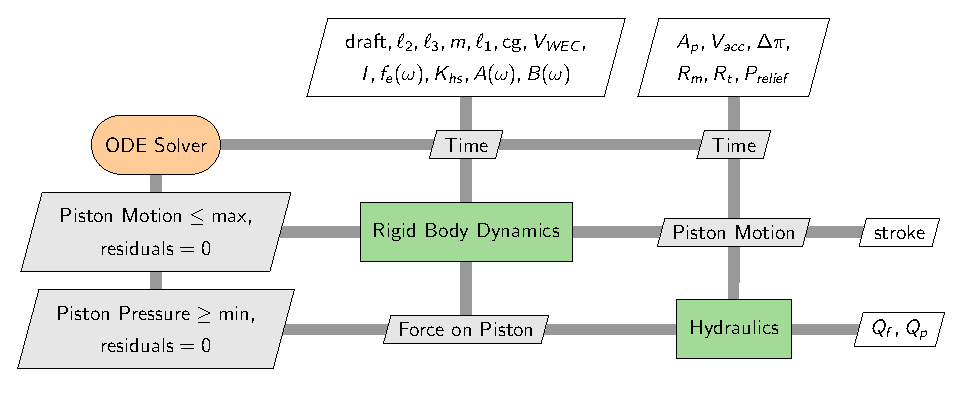
\includegraphics[width=0.8\linewidth]{../figs/xDSM_sysdyn.pdf}
    \captionof{figure}{xDSM diagram of the system dynamics module.}
    \label{fig:sysdynxdsm}
\end{figure*}

\subsubsection{Rigid Body Dynamics}
The rigid body dynamics module considers the OSWEC dynamics as well as the dynamics of the mechanism connecting the WEC to the piston. The OSWEC dynamics are governed by Equation \ref{eq:wec}, with the various hydrodynamic coefficients determined through the BEM solver, as discussed in Section \ref{sec:hydro}. WEC-Sim \cite{wecsim}, an open-source software developed by the National Renewable Energy Laboratory (NREL) and Sandia National Laboratories, then uses these coefficients to solve the WEC dynamics in the time domain. The mechanism is modeled using the Simscape multibody toolbox, this models the kinematics and dynamics of the mechanism, relating the OSWEC pitch motion to the linear motion of the piston, as well as the force on the piston to the torque at the OSWEC hinge.

\subsubsection{Hydraulics}
The hydraulic circuit (Figure \ref{fig:hydraulics}) is modeled using the  isothermal liquid domain from the Simscape fluids toolbox. This domain is well suited for modeling hydraulic systems. A high level view of the Simscape model is shown in Figure \ref{fig:hydraulic_simscape}. This high level view shows the key components of the hydraulic circuit. The ``Piston Cylinder'' models the piston and directional valves. Flow out of the ``Piston Cylinder'' then passes through the accumulator, pressure relief valve, the ``RO Subsystem'' (which models the SWRO membrane), and finally the throttle valve on the brine side. 

\begin{figure*}  % The [t] option places the figure at the top of the page
    \centering
    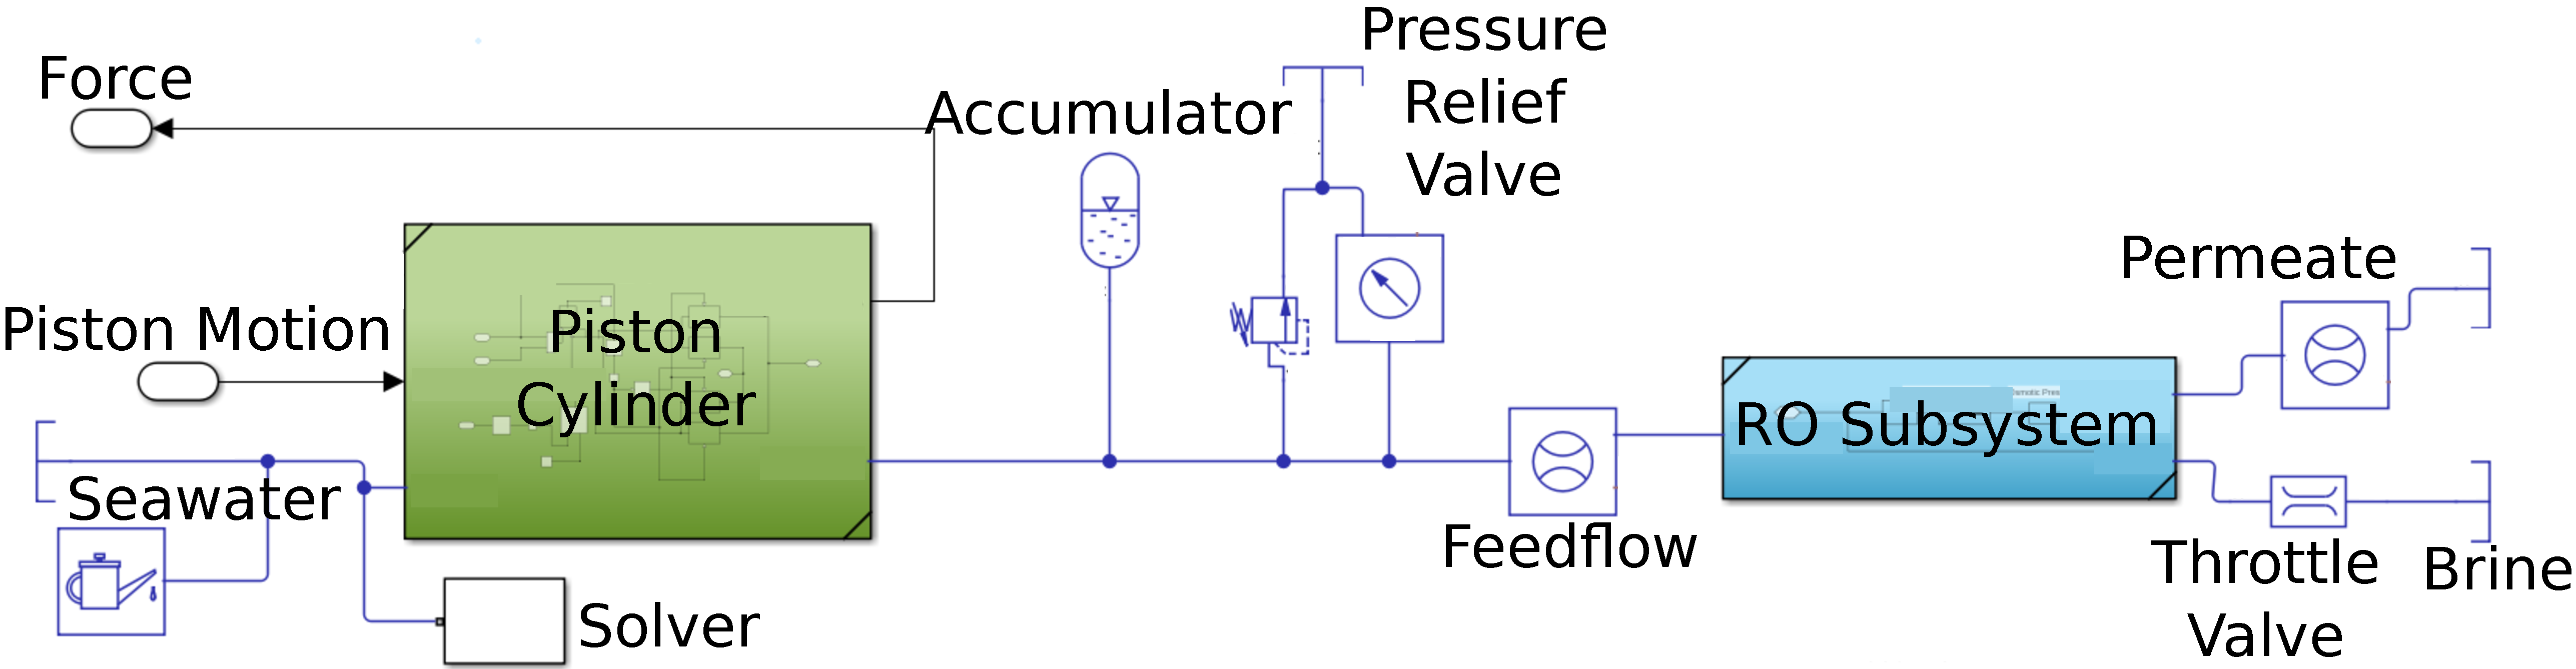
\includegraphics[width=0.7\linewidth]{../figs/simscape_hydraulics.pdf}
    \captionof{figure}{Simscape model of the hydraulic circuit.}
    \label{fig:hydraulic_simscape}
\end{figure*}

The ``Piston Cylinder'' is modeled similarly to the model used by Yu and Jenne (2018) \cite{Yu2018}. The only notable difference is the use of the isothermal liquid domain rather than the hydraulics domain. 

The ``RO Subsystem'' model is shown in Figure \ref{fig:ro_simscape}. The check valve prevents forward osmosis, and the membrane resistance block combined with the osmotic pressure block create a Simscape representation of Equation \ref{eq:ro}.

\begin{figure}[h]
    \centering
    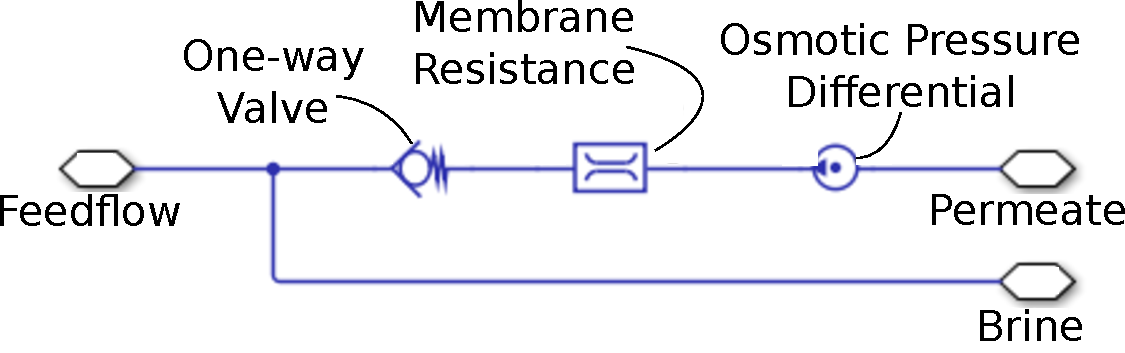
\includegraphics[width=0.7\linewidth]{../figs/simscape_ro.pdf}
    \captionof{figure}{Simscape model of the RO membrane.}
    \label{fig:ro_simscape}
\end{figure}

\subsection{Economics} \label{sec:econ}
Our objective function is an adaptation of the levelized cost of energy (LCOE) [\$/kWh] function used by the U.S. Department of Energy \cite{LCOE_DOE}. Annual water production (AWP) [m$^3$/yr] in substituted in for annual energy production [kWh/yr], creating this function for levelized cost of water (LCOW) [\$/m$^3$]:
\begin{equation}
    \text{LCOW} = \frac{(\text{FCR}\times\text{CAPEX}) + \text{OPEX}}{\text{AWP}},
    \label{eq:LCOW}
\end{equation}
\noindent The fixed charge rate, FCR, is set to 10.8\% as assumed in the U.S. Department of Energy report \cite{LCOE_DOE}. Annual water production (AWP) is calculated by scaling the results of the system dynamics simulation to a yearly basis. The costs are then split into capital expenditures (CAPEX) [\$] and annual operating expenses (OPEX) [\$/yr].

To determine both CAPEX and OPEX, expenses are broken down into three cost models, WEC, PTO, and SWRO plant. These cost models are not indented to provide exact cost estimates. Rather, they are intended to quantify the relative costs of different designs to guide the optimization process. Although these cost models are not comprehensive, they serve as a tool to highlight the impact of MDO for wave-driven desalination systems. Each cost model is discussed in the following sections. Note that all costs are reported in 2025 USD.

\subsubsection{WEC Cost Model}
WEC cost modeling is challenging due to limited real world data, limiting accuracy. Despite the this challenge, a practical cost model that captures key trends for design comparison is possible. In this study, we follow the approach used by Grasberger et al. (2024) \cite{Grasberger2024} in their OSWEC CCD study. This model defines cost as a function of the float's surface area:
\begin{equation}
    \text{Cost} = C_{1,ref}\left(\frac{A_{x}}{A_{ref}}\right) + C_{2,ref}\left(1 + \text{log}\left(\frac{A_{x}}{A_{ref}}\right)\right),
\end{equation}
\noindent where $A_{x}$ [m$^2$] is the float surface area and $A_{ref}$ [m$^2$] is the reference float surface area. $C_{1,ref}$ [\$] and $C_{2,ref}$ [\$] are the costs of the reference float associated with the two terms. Structural components are captured in the linear term while other expenses that are less dependent on size are captured in the logarithmic term. This cost model is dependent on accurate reference costs to make meaningful comparisons. For this study, reference costs are taken from NREL's Reference Model 5 (RM5) \cite{rm5}. The costs from this reference model are tailored to this study by excluding the costs of irrelevant components, such as the electrical PTO system. Many transit and other overhead costs are also excluded as they are unlikely to scale with WEC size. 

At small WEC sizes, it is possible for the logarithmic term to become negative, which is unrealistic. To avoid this, a minimum $C_2$ cost is used when the equation drops below this threshold. For this study, this minimum $C_2$ cost is set to \$0 for both CAPEX and OPEX.

\subsubsection{PTO Cost Model}
The PTO cost covers the hydraulic cylinder and accumulator. The accumulator cost is estimated as a function of accumulator volume ($V_{acc}$):
\begin{equation}
    \text{Cost} = 1.621 \times 10^5 V_{acc} ^{0.986},
\end{equation}
\noindent where the constants are tuned to approximate supplier quotes \cite{reasontek}. 

The hydraulic cylinder cost is a function of the required amount of steel:
\begin{equation}
    \text{Cost} = C_{\text{316}} \rho_{\text{316}} V_{\text{316}} (1+L),
\end{equation}
\noindent where $C_{\text{316}}$ [\$/lb] is the unit cost of 316 stainless steel, $\rho_{\text{316}}$ [lb/in$^3$] is the density of 316 stainless steel, $V_{\text{316}}$ [in$^3$] is the volume of 316 stainless steel required, and $L$ [-] is a labor multiplier. The volume required is the sum of the required volumes for the various parts of the cylinder: the cylinder barrel ($V_{\text{cylinder}}$) [in$^3$], the end caps ($V_{\text{cap}}$) [in$^3$], the piston head ($V_{\text{piston}}$) [in$^3$], and the piston rod ($V_{\text{rod}}$) [in$^3$].
\begin{equation}
    V_{\text{316}} = V_{\text{cylinder}} + 2V_{cap} + V_{\text{piston}} + V_{text{rod}},
\end{equation}
The thicknesses of the cylinder barrel and end caps are calculated according to the ASME Boiler and Pressure Vessel Code \cite{ASME_BPVC}. The piston head uses the same thickness as the end caps, while the piston rod diameter is set to avoid buckling and tensile/compressive failure. The required stroke length, which is needed for the cylinder volume calculation, is determined from the system dynamics simulation.

\subsubsection{SWRO Cost Model}
SWRO plant cost models on the scale of this paper (producing thousands of m$^3$/day) are scarce and poorly documented. Most well documented cost models focus on large-scale plants (hundreds of thousands of m$^3$/day) \cite{Slocum2016,Haefner2023,roopexcurve,Wittholz2008}, and are therefore not suitable for this study. Studies that examine plants of comparable size typically lack transparent cost models \cite{Elkadeem2024,Goekcek2016,DEEP5manual}. 

This study aims to use a transparent cost model for small-scale SWRO plants. Voutchkov's \emph{Desalination Project Cost Estimating and Management} \cite{voutch} provides cost curves for CAPEX (section 4) and OPEX (section 5) for a wide range of plant sizes. Using different curves can be used to model different plant architectures, giving this model additional flexibility. In this study, each curve is fitted to a power function, which prevents unrealistic behavior at the lower end of the scale.

\section{Results} \label{sec:results}


\section{Discussion} \label{sec:discussion}


\section{Conclusion and Future Work} \label{sec:conclusion}


\bibliographystyle{elsarticle-num}  % choose a style
\bibliography{refs}                 % points to refs.bib

\appendix
\newpage
\section{TABLES OF PARAMETERS} \label{app:params}

\begin{table}[h]
    \centering
    \caption{GENETIC ALGORITHM HYPERPARAMETERS}
    \begin{tabular}{ccc}
        \hline
        \textbf{Parameter} & \textbf{Value} & \textbf{Units} \\
        \hline
        population size & 256 & - \\
        number of generations & 300 & - \\
        mutation rate & 0.02 & - \\
        crossover rate & 0.8 & - \\
        number of elites kept & 3 & - \\
        tournament size & 4 & - \\
        bits per variable & 8 & - \\ 
        \hline
    \end{tabular}
    \label{tab:paramsga}
\end{table}


\begin{table}[h]
    \centering
    \caption{GENERAL PARAMETERS}
    \begin{tabular}{ccc}
        \hline
        \textbf{Parameter} & \textbf{Value} & \textbf{Units} \\
        \hline
        gravitational acceleration & 9.81 & m/s$^2$ \\
        ocean density & 1025 & kg/m$^3$ \\
        distance to shore & 500 & m \\
        ocean temperature & 298.15 & K \\
        water depth & 12 & m \\
        wave direction & 0 \cite{Yu2018} & degrees \\
        
        wave spectrum & Pierson–Moskowitz \cite{Yu2018} & -  \\
        significant wave height & 2.64 \cite{Yu2018} & m \\
        peak period & 9.86 \cite{Yu2018} & s \\

        Fixed Charge Rate & 10.8 \cite{LCOE_DOE} & \% \\
        \hline
    \end{tabular}
    \label{tab:paramsgeneral}
\end{table}


\begin{table}[h]
    \centering
    \caption{SWRO PARAMETERS}
    \begin{tabular}{ccc}
        \hline
        \textbf{Parameter} & \textbf{Value} & \textbf{Units} \\
        \hline
        feedflow total dissolved solids & 35946 \cite{Yu2018} & mg/L \\
        permeate total dissolved solids & 150 \cite{Yu2018} & mg/L \\
        salt molar weight & 58.44 & g/mol \\
        water permeability coefficient & $2.57\times10^{-12}$ \cite{Yu2018} & m$^3$/N-s \\
        recovery ratio & 44.2 \cite{wave} & \% \\
        single SW30HR-380 area & 35 \cite{SW30HR380} & m$^2$ \\
        single SW30HR-380 flow rate & 24.6 \cite{SW30HR380} & m$^3$/day \\
        \hline
    \end{tabular}
    \label{tab:paramsswro}
\end{table}

\begin{table}[h]
    \centering
    \caption{WEC PARAMETERS}
    \begin{tabular}{ccc}
        \hline
        \textbf{Parameter} & \textbf{Value} & \textbf{Units} \\
        \hline
        draft & 9 & m \\
        cg draft factor & -0.7778 & - \\
        unit inertia & 14.57 & m$^2$ \\
        RM5 surface area & 1214 \cite{rm5} & m$^2$ \\
        RM5 flap cost & 3364648.63 \cite{rm5} & \$ \\
        RM5 base cost & 1706415.27 \cite{rm5} & \$ \\
        RM5 bearings cost & 17420.34 \cite{rm5} & \$ \\
        RM5 mooring cost & 997819.2 \cite{rm5} & \$ \\
        RM5 monitoring cost & 616480.27 \cite{rm5} & \$/yr \\
        RM5 marine operations cost & 101387.23 \cite{rm5} & \$/yr \\
        RM5 shore operations cost & 347280.29 \cite{rm5} & \$/yr \\
        RM5 parts cost & 86237.2 \cite{rm5} & \$/yr \\
        RM5 consumables cost & 17480.19 \cite{rm5} & \$/yr \\
        RM5 insurance rate & 2 \cite{rm5} & \% \\
        \hline
    \end{tabular}
    \label{tab:paramswec}
\end{table}

\begin{table}[h]
    \centering
    \caption{PTO PARAMETERS}
    \begin{tabular}{ccc}
        \hline
        \textbf{Parameter} & \textbf{Value} & \textbf{Units} \\
        \hline
        $\ell_2$ & 4.7 & m \\
        $\ell_3$ & 0 & m \\
        max piston stroke & 20 & m \\
        SS316 cost & 2.00 \cite{316ss} & \$/in$^3$ \\
        SS316 density & 0.29 \cite{316ss} & lb/in$^3$ \\
        SS316 yield strength & 206 \cite{316ss} & MPa \\
        SS316 Young's modulus & 164 \cite{316ss} & GPa \\
        cylinder factor of safety & 6 & - \\
        rod factor of safety & 1.5 & - \\
        labor factor & 0.7 & - \\
        end cap attachment factor & 0.3 \cite{ASME_BPVC} & - \\
        cylinder joint efficiency & 0.8 \cite{ASME_BPVC} & - \\
        \hline
    \end{tabular}
    \label{tab:paramspto}
\end{table}

\begin{table}[h]
    \centering
    \caption{SOLVER PARAMETERS}
    \begin{tabular}{ccc}
        \hline
        \textbf{Parameter} & \textbf{Value} & \textbf{Units} \\
        \hline
        BEM frequencies & 0.2, 0.34, 0.48, ..., 3& rad/s \\
        SysDyn time step & 0.1 & s \\
        SysDyn sim time & 300 & s \\
        \hline
    \end{tabular}
    \label{tab:paramssolve}
\end{table}


\end{document}

